\documentclass[conference]{IEEEtran}
\IEEEoverridecommandlockouts

\usepackage{amsmath,amssymb,amsfonts}
\usepackage{graphicx}
\usepackage{textcomp}
\usepackage{xcolor}
\usepackage{booktabs}
\usepackage{multirow}
\usepackage{cite}
\usepackage{url}
\usepackage[hidelinks]{hyperref}

\newcommand{\MG}{\mathrm{MG}}
\newcommand{\AUC}{\mathrm{AUC}}

\begin{document}

\title{Masking or Noise? Null-Calibrated Auditing of Per-Dimension Failures Behind Composite Wellness Scores in Federated Learning}

\author{\IEEEauthorblockN{Anonymous Authors}}

\maketitle

\begin{abstract}
Consumer wellness apps combine several health dimensions, such as sleep, activity and mood, into one composite score, and the composite can look fine while one dimension fails. We introduce the Masking Gap to measure this: the average of the per-dimension areas under the receiver operating characteristic curve minus the lowest one. The Masking Gap is never negative, and under federated learning it must be estimated on each client's small test set, so a raw value can be pure noise. We therefore derive its distribution under chance, report how far an observed gap exceeds chance, and set severity tiers from that distribution. We study 20 income-by-age clients built from the 2015--2018 National Health and Nutrition Examination Survey (8,353 adults, seven dimensions) in two stages. In a baseline stage with nine centralized, federated and per-dimension training conditions, the per-client gap (0.106--0.117) was close to its chance level (0.103), and detecting a gap of 0.10 would need about 300 test records per client. A full protocol then ran all nine conditions and FedProx with validation-based model selection, tuned learning rates, ten seeds, class-weighted and focal losses, a leakage-audited 38-column feature set and three client partitions. Two real failures emerged. First, federated outputs at chance in the baseline were caused by unscaled inputs; after standardization, federated averaging trailed centralized training by only 0.008 in area under the curve averaged over dimensions (at most 0.013 on any dimension). Second, in every full-protocol configuration the composite score was worse than each dimension's own output at flagging that dimension's poor cases, by 0.02--0.16 in area under the curve. Near-zero sensitivity for sleep and depression at the default threshold was a threshold artifact (0.51--0.70 at validation-tuned thresholds). We end with practical recommendations for auditing composite health models trained with federated learning.
\end{abstract}

\begin{IEEEkeywords}
composite health scores, federated learning, model auditing, multi-task learning, permutation test, wellness applications
\end{IEEEkeywords}

\section{Introduction}

Consumer wellness platforms summarize sleep, activity, mental health and other dimensions in a single composite score, usually a proprietary weighted average~\cite{doherty2025,whoop2024,garmin2024,oura2024}. A good composite can hide a poor dimension. This already happens in the labels: among adults in the 2015--2018 National Health and Nutrition Examination Survey (NHANES)~\cite{nhanes2015}, 35.2\% of those sleeping under seven hours and 18.6\% of those screening positive for depression (PHQ-9 $\geq$ 10) still have a composite (here, the share of seven dimensions not flagged poor) at or above the median. When a learned model produces the composite, the question becomes: does the model fail on one dimension while the overall score still looks fine?

Federated learning (FL) makes this question both more important and harder to answer. Wellness data are private and differ across demographic groups~\cite{rieke2020}, so models are trained across sites that keep their data, and an auditor usually sees only each client's per-dimension results. We call a dimension \emph{masked} when the model predicts it clearly worse than the others while overall performance still looks acceptable. We know of no statistic for this, so we introduce one, the \emph{Masking Gap} (MG): for each client, the average of the per-dimension areas under the ROC curve (AUCs) minus the smallest of them. The average is what an overall report conveys; the minimum is the dimension it can hide. A client whose seven AUCs average 0.65 while its worst sits at 0.50 has MG = 0.15.

MG is easy to compute, but it has a built-in flaw. A minimum never exceeds a mean, so MG is never negative, and federated clients have small test sets, so even a model with no skill produces a sizable MG. A raw MG therefore means little on its own. An auditor needs to know how large MG is \emph{when no dimension is actually failing}, and how far the observed MG exceeds that.

We study this with 20 income-by-age clients built from NHANES, in two stages. A \emph{baseline} stage trains nine conditions (centralized training, six FL aggregation schemes and two variants that train each dimension separately) with a simple pipeline: six raw inputs, one learning rate, three seeds and the final model evaluated. A \emph{full protocol} then runs all nine, plus FedProx, with validation-based model selection, standardized inputs, tuned learning rates, ten seeds, losses for class imbalance, a richer leakage-audited feature set and three client partitions. The baseline shows how a raw statistic misleads and what a per-dimension audit catches; the full protocol tests which findings survive careful training. Our contributions:

\begin{enumerate}
\item \textbf{A calibrated masking audit.} We introduce MG and derive its distribution under chance (its \emph{null}), exactly from each client's class counts and by permuting labels. From the null we report the \emph{MG-excess} (observed MG minus its chance level), severity tiers, and the test size a client needs to detect a gap of a given size.
\item \textbf{Per-client MG in the baseline is mostly noise.} Across the nine baseline conditions (20 clients, 3 seeds), per-client MG (0.106--0.117) is close to its chance level (0.103); no condition differs after Holm correction, and 90\% of client results lie within noise. A real excess appears in every condition only with richer features, and it is small ($\approx$0.02, a fifth of the raw MG).
\item \textbf{Two real failures that the composite hides.} A per-dimension audit finds federated outputs at chance in the baseline (Sleep and Mental AUC $\approx$0.5), caused by unscaled inputs; after standardization, FedAvg trails centralized training by 0.008 macro-AUC (AUC averaged over dimensions; at most 0.013 on any dimension). Separately, a second statistic we introduce, the \emph{composite blind spot} $\Delta_d$, measures how much AUC a dimension loses when only the composite is shown. It is positive in every full-protocol configuration ($\Delta_d$ = 0.02--0.16 AUC, all CIs above zero).
\item \textbf{Robustness.} Near-zero sensitivity for Sleep and Mental at the default 0.5 threshold is a threshold artifact (tuned sensitivity 0.51--0.70). No FL scheme or per-dimension variant changes pooled MG (class weighting lowers it only by lowering AUC), the results hold under three client partitions, and one global threshold leaves income-group sensitivity gaps of up to 0.86.
\end{enumerate}

\section{Related Work}

\emph{FL for health.} FedAvg (McMahan et al.~\cite{mcmahan2017}) trains a shared model by averaging locally computed updates; differences between sites are the main obstacle in health deployments~\cite{rieke2020,grataloup2024}. Remedies change how updates are aggregated: proximal regularization (FedProx, Li et al.~\cite{li2020fedprox}), control variates (SCAFFOLD, Karimireddy et al.~\cite{karimireddy2020}), personalization (Ditto, Li et al.~\cite{li2021ditto}; Fallah et al.~\cite{fallah2020}), loss-based reweighting for fairness (q-FedAvg, Li et al.~\cite{li2020qfedavg}) and trust weighting by the cosine similarity of client updates (FLTrust, Cao et al.~\cite{cao2021fltrust}). All target differences between clients on a single objective; none checks differences between output dimensions within a client.

\emph{Aggregate metrics hide subgroup failures.} An overall metric can hide failures on clinically important subsets~\cite{oakdenrayner2020} or groups~\cite{obermeyer2019}, so evaluations should report results by subgroup and quantify uncertainty~\cite{burnell2023,collins2024}. Composite scores are now common in consumer wearables~\cite{doherty2025}. We apply the same idea to the dimensions of a composite score: we introduce a statistic for the gap between them and give it the chance baseline that small federated clients need.

\emph{Multi-task training.} When several task losses are summed, the tasks can conflict~\cite{sener2018} and some can dominate training~\cite{chen2018gradnorm}; loss balancing~\cite{chen2018gradnorm,kendall2018} and gradient surgery~\cite{yu2020pcgrad} reduce this. Class imbalance makes it worse; focal loss~\cite{lin2017focal} and class weighting are standard remedies and serve as baselines here.

\emph{AUC uncertainty and permutation tests.} An AUC gets noisier as the smaller class shrinks~\cite{hanley1982}. The minimum of several noisy AUCs is therefore biased downward, which biases MG upward. Permuting labels gives an exact null for classifier performance when scores carry no information~\cite{ojala2010}; we use it per client and for the whole population.

\section{Data and Methods}

\subsection{Cohort, dimensions and clients}

NHANES samples the U.S.\ civilian non-institutionalized population. Of the 19,225 participants in the 2015--2016 and 2017--2018 cycles, 11,848 were adults, and 8,353 (aged 18--80) had valid inputs and labels. We do not apply survey weights, so prevalences describe this sample, not the U.S.\ population. Table~\ref{tab:dims} defines the seven binary ``poor'' labels. Each uses a published cut-point except Diet, which uses the sample median because no guideline exists for total (as opposed to added) sugar. Clients combine five poverty-income-ratio bands ($<$1, 1--2, 2--3, 3--4, $\geq$4) with four age bands (18--35, 36--50, 51--64, $\geq$65), giving 20 clients of 183--702 records. Each seed draws an 80/20 train/test split stratified by client, so a client's test set holds only 37--141 records.

\begin{table}[t]
\caption{Wellness dimensions (analytic sample, $n=8{,}353$). Activity: total MET-min/week over work, transport and leisure, scored as in the WHO GPAQ guide~\cite{gpaq} (vigorous 8 MET, moderate 4 MET); 600 MET-min equals the WHO minimum of 150 min of moderate activity per week~\cite{who2020}. Sedentary: PAD680 is total daily sitting, while the 6 h cut-point comes from leisure-time sitting~\cite{patel2010}, so this anchor is approximate. Prev.: share flagged poor. Eval.: clients (of 20) whose test set has $\geq$5 positives and $\geq$5 negatives, range over the three baseline seeds.}
\label{tab:dims}
\centering\small
\setlength{\tabcolsep}{1.8pt}
\begin{tabular}{@{}llllr@{\hspace{6pt}}c@{}}
\toprule
Dimension & Variable & Poor if & Anchor & Prev. & Eval. \\
\midrule
Sleep & SLD012 & $<$7 h/night & \cite{watson2015} & 23.5\% & 20 \\
Activity & PAQ MET & $<$600 MET-min/wk & \cite{who2020} & 36.5\% & 20 \\
Sedentary & PAD680 & $>$360 min/day & \cite{patel2010} & 36.1\% & 20 \\
Mental & PHQ-9 & score $\geq$10 & \cite{kroenke2001} & 8.2\% & 11--14 \\
Metabolic & BMXBMI & BMI $\geq$30 & \cite{who2000} & 41.5\% & 20 \\
Wellbeing & HSD010 & fair/poor & \cite{idler1997} & 23.8\% & 17--19 \\
Diet & DR1TSUGR & $>$ median sugar & --- & 50.0\% & 20 \\
\bottomrule
\end{tabular}
\end{table}

\subsection{Training}

All conditions use the same neural network: a shared 128--64 ReLU backbone with seven sigmoid outputs, one per dimension, trained with Adam~\cite{kingma2015}, batch size 32 and the unweighted sum of the seven binary cross-entropy losses.

Both stages share this network, the clients and, for each seed, the test set.

\emph{Baseline stage.} Six unscaled inputs: age, sex, poverty-income ratio, race/ethnicity code, and mean systolic and diastolic blood pressure. Learning rate $10^{-3}$, seeds 42, 123 and 456, and the final model is evaluated. Nine conditions, C1--C8 in Table~\ref{tab:conds}. Centralized models train for 150 epochs; federated conditions use 50 rounds of 3 local epochs.

\begin{table}[t]
\caption{Training conditions. In the baseline, Ditto, q-FedAvg and CS-Agg use $\lambda{=}0.1$, $q{=}1$ and 10 warm-up rounds; the full protocol tunes them.}
\label{tab:conds}
\centering\small
\setlength{\tabcolsep}{3pt}
\begin{tabular}{@{}lp{0.79\columnwidth}@{}}
\toprule
C1 & Centralized training, one network with seven outputs \\
C2 & Seven separate centralized single-output networks \\
C2-FL & Seven separate single-output FedAvg federations \\
C3 & FedAvg: local updates averaged by client size (McMahan et al.~\cite{mcmahan2017}) \\
C4 & SCAFFOLD: control variates correct client drift (Karimireddy et al.~\cite{karimireddy2020}); Adam steps in the baseline, SGD in the full protocol \\
C5 & CS-Agg: after plain warm-up rounds, each client is weighted by the mean cosine similarity of its update to the other clients' updates (shifted to be non-negative, normalized) \\
C6 & Ditto: personalized client models pulled toward the global model (Li et al.~\cite{li2021ditto}) \\
C7 & q-FedAvg: clients with higher loss weighted more (Li et al.~\cite{li2020qfedavg}) \\
C8 & FedAvg in which each local batch takes seven separate update steps, one per dimension \\
C9 & FedProx: proximal term toward the global model (Li et al.~\cite{li2020fedprox}); full protocol only \\
+cw, +focal & C1 or C3 with class-weighted or focal loss; full protocol only \\
\bottomrule
\end{tabular}
\end{table}

\emph{Full protocol.} We hold out 12.5\% of the training data (10\% overall, stratified by client) for validation and evaluate the checkpoint (every 5 epochs, or every round) with the best validation macro-AUC; C2-FL picks the round for each dimension separately. Continuous inputs are standardized and race/ethnicity is one-hot encoded, using training-set statistics only; under FL, clients would share global means and variances, which secure aggregation of sums can provide. The learning rate is tuned once on a separate seed (2026) and then fixed. The grid starts at $\{3{\times}10^{-3}, 10^{-3}, 3{\times}10^{-4}, 10^{-4}\}$ and is widened by a half-decade whenever the best value lies at its edge, until it is interior, which it is for every condition. We use ten evaluation seeds; since each draws a different client-stratified split, this is repeated random-subsampling cross-validation.

We run all nine conditions with these settings. SCAFFOLD takes plain local SGD steps (grid $\{0.3, 0.1, 0.03, 0.01\}$), as its control-variate update assumes. We add FedProx (C9, Li et al.~\cite{li2020fedprox}), tuning its proximal weight $\mu \in \{0.001, 0.01, 0.1\}$ with the learning rate. Ditto's $\lambda \in \{0.01, 0.1, 1\}$, q-FedAvg's $q \in \{0.1, 1, 5\}$ and CS-Agg's warm-up $\in \{5, 10, 20\}$ rounds are tuned on the same seed at the selected learning rate. We also run C1 and C3 with two losses for class imbalance: class-weighted cross-entropy (positive weight $n^-/n^+$ per dimension, computed by each client, capped at 20) and focal loss ($\gamma{=}2$)~\cite{lin2017focal}.

\emph{Inputs and partitions.} We compare the six base inputs (11 columns after encoding) with an \emph{enriched} set of 38 columns that adds education, marital status, household size, U.S.\ birth, pulse, HbA1c, total and HDL cholesterol, smoking status, insurance, routine care, care visits, hospitalization, diagnosed diabetes, hypertension, high cholesterol, asthma, cardiovascular disease and cancer, and prescription count. All are measured on the full exam sample, so no client shrinks. To prevent leakage, no variable comes from a questionnaire or exam component that defines a label (SLQ, PAQ/PAD, DPQ, BMX, HSQ and HUQ010, DR1/DR2). Besides the income-by-age clients, FedAvg is trained on two other partitions with the same test sets: a fixed random split into 20 equal clients (no heterogeneity) and 12 race/ethnicity $\times$ sex clients. Centralized predictions are regrouped by the same clients.

\subsection{Measures}

\emph{Per-dimension AUC.} For client $c$ and dimension $d$, $\AUC_{c,d}$ is the probability that a randomly chosen poor case gets a higher predicted risk than a randomly chosen non-poor case (0.5 = chance). We compute it only when the client's test set has at least 5 cases of each class; otherwise the dimension is left out of that client's statistics.

\emph{Masking Gap.} For client $c$, over the dimensions $E_c$ with a computable AUC, we define
\begin{equation}
\MG_c = \frac{1}{|E_c|}\sum_{d\in E_c}\AUC_{c,d} - \min_{d\in E_c}\AUC_{c,d} \;\geq\; 0 .
\end{equation}
MG is zero when all dimensions are predicted equally well and grows as the worst falls behind the average. We compute it per client, as an FL audit would, and on the pooled test set (population level, below).

\emph{Calibrating MG against chance.} Under the null hypothesis $H_0$ that scores carry no information about any label, the ranks of the $k$ positives among $n$ records are a uniformly random subset. We draw $10^4$ null AUCs per client, seed and dimension from its exact $(k,n)$ (\emph{random-score null}, used for the baseline) and, for the full protocol, shuffle test rows jointly across all seven labels $10^3$ times (\emph{label-permutation null}, which keeps the correlation between labels)~\cite{ojala2010}. We report $\text{MG-excess}_c = \MG_c - \mathbb{E}_0[\MG_c]$, the observed MG minus its chance level, which can be negative, and the percentile of $\MG_c$ within its null. Severity tiers come from the null instead of fixed cut-points: \emph{within noise} (below the 95th null percentile), \emph{elevated} (95th--99th) and \emph{severe} ($\geq$ 99th). By chance alone, 5\% and 1\% of clients fall in the upper two tiers.

\emph{A closed form for planning.} Under $H_0$, a dimension's AUC has mean 0.5 and variance $\sigma_d^2 = (n+1)/(12\,k_d(n-k_d))$, the null variance of the Mann--Whitney statistic~\cite{mann1947} divided by $(k_d(n-k_d))^2$, which is close to normal for moderate $n$. Treating the $K$ dimensions as independent with a common $\bar\sigma^2 = \frac{1}{K}\sum_d \sigma_d^2$ gives
\begin{equation}
\mathbb{E}_0[\MG] \approx c_K\,\bar\sigma, \qquad q_{0.95}[\MG] \approx c'_K\,\bar\sigma ,\label{eq:closed}
\end{equation}
where $c_K$ and $c'_K$ are the mean and 95th percentile of (mean $-$ min) of $K$ standard normals ($c_7 = 1.35$, $c'_7 = 2.27$). With prevalences $p_d$, $\bar\sigma^2 \approx \frac{1}{12n}\cdot\frac{1}{K}\sum_d \frac{1}{p_d(1-p_d)}$, so a client needs about $n \approx (c'_K/g)^2\,\frac{1}{12K}\sum_d \frac{1}{p_d(1-p_d)}$ test records before a gap $g$ exceeds chance at the 5\% level. No simulation is needed.

\emph{Population level.} We also compute each dimension's AUC on the pooled test set (1,671 records) and the pooled MG with its permutation null; for the baseline, we report the client-averaged AUC per dimension with a 95\% cluster-bootstrap CI over clients.

\emph{Composite blind spot.} MG compares dimensions with each other; it does not measure what the composite itself hides. For that we introduce a second statistic. Let $s_i = \frac{1}{7}\sum_d p_{i,d}$ be the composite risk a user would see. For dimension $d$,
\begin{equation}
\Delta_d = \AUC(p_{\cdot,d}; y_{\cdot,d}) - \AUC(s; y_{\cdot,d})
\end{equation}
is the AUC lost when only the composite is shown. $\Delta_d$ can be negative, if averaging correlated outputs detects dimension $d$ better than its own output does. A positive $\Delta_d$ is the expected direction; what an audit needs is its size, for which dimensions it is large, and whether any training scheme removes it.

\emph{Thresholds and calibration.} For each dimension we report sensitivity (true-positive rate, TPR), false-positive rate and balanced accuracy at a 0.5 threshold and at a threshold chosen on validation data by Youden's $J$~\cite{youden1950}, plus AUPRC (compared with prevalence), Brier score and expected calibration error (ECE, 10 bins).

\emph{Subgroup fairness.} For each dimension we compute AUC within each income band and age band, the worst-group AUC, the largest between-group AUC gap, and the between-group TPR gap at the tuned threshold (equal opportunity~\cite{hardt2016}).

\emph{Statistics.} Client-level MG analyses treat the client as the unit (averaged over seeds, $n{=}20$), with 95\% CIs from a cluster bootstrap over clients, two-sided Wilcoxon signed-rank tests~\cite{wilcoxon1945}, Hodges--Lehmann effect sizes and Holm correction~\cite{holm1979} within each family of tests. A linear mixed model $\MG \sim \text{condition} + \text{seed} + (1\,|\,\text{client})$ serves as a sensitivity analysis. In the full protocol, pooled metrics are averaged over seeds with 95\% bootstrap CIs over seeds, and conditions are compared with paired $t$-tests over seeds ($n{=}10$, $t$-based 95\% CIs, Holm correction within each metric).

\section{Results}

We report the baseline stage first (Sections IV-A and IV-B) and then the full protocol.

\subsection{Baseline: per-client Masking Gap is mostly noise}

Table~\ref{tab:baseline} compares per-client MG in the nine baseline conditions with its chance level. Average per-client MG ranges from 0.106 to 0.117, yet a model with no information about any label would score 0.103 on the same test sets. MG-excess lies between $+0.002$ and $+0.013$, about a tenth of the raw MG, and no condition differs from chance after Holm correction (smallest adjusted $p = 0.27$). Of all 540 client--seed--condition results, 8.0\% are \emph{elevated} and 1.7\% \emph{severe}, against the 5\% and 1\% that chance predicts (Fig.~\ref{fig:null}b): a small real excess may exist, but it is too small to attribute to any condition.

The simplest way to read MG would be with fixed cut-points, for example moderate at 0.10 and severe at 0.20. These sit near the median (0.10) and upper tail (95th percentile 0.13--0.24, depending on client) of the null, so they label noise as masking: under them, 52\% of the baseline results would be moderate or worse, whereas under calibrated tiers 90\% are within noise.

\begin{table}[t]
\caption{Baseline conditions compared with chance (3 seeds). MG-excess: mean over clients of MG minus its random-score null mean, with 95\% cluster-bootstrap CI. $p$: two-sided Wilcoxon test against 0, Holm-adjusted across conditions. $>$p95: share of client--seed results above their null 95th percentile (5\% expected by chance).}
\label{tab:baseline}
\centering\small
\setlength{\tabcolsep}{1.8pt}
\begin{tabular}{@{}lccrcc@{}}
\toprule
Condition & MG & Null & MG-excess [95\% CI] & $p$ & $>$p95 \\
\midrule
C1 Centralized     & 0.107 & 0.103 & $+0.004$ [$-0.007$, $0.015$] & 1.00 & 6.7\% \\
C2 Sep.\ classif.  & 0.108 & 0.103 & $+0.005$ [$-0.006$, $0.017$] & 1.00 & 6.7\% \\
C2-FL Fed.\ sep.   & 0.106 & 0.103 & $+0.002$ [$-0.011$, $0.016$] & 1.00 & 11.7\% \\
C3 FedAvg          & 0.116 & 0.103 & $+0.012$ [$0.003$, $0.022$] & 0.35 & 6.7\% \\
C4 SCAFFOLD        & 0.109 & 0.103 & $+0.006$ [$-0.004$, $0.015$] & 1.00 & 10.0\% \\
C5 CS-Agg          & 0.117 & 0.103 & $+0.013$ [$0.004$, $0.023$] & 0.27 & 11.7\% \\
C6 Ditto           & 0.113 & 0.103 & $+0.010$ [$0.000$, $0.020$] & 0.63 & 8.3\% \\
C7 q-FedAvg        & 0.113 & 0.103 & $+0.009$ [$-0.003$, $0.022$] & 1.00 & 11.7\% \\
C8 Per-dim.        & 0.111 & 0.103 & $+0.008$ [$0.000$, $0.016$] & 0.63 & 13.3\% \\
\bottomrule
\end{tabular}
\end{table}

\begin{figure}[t]
\centering
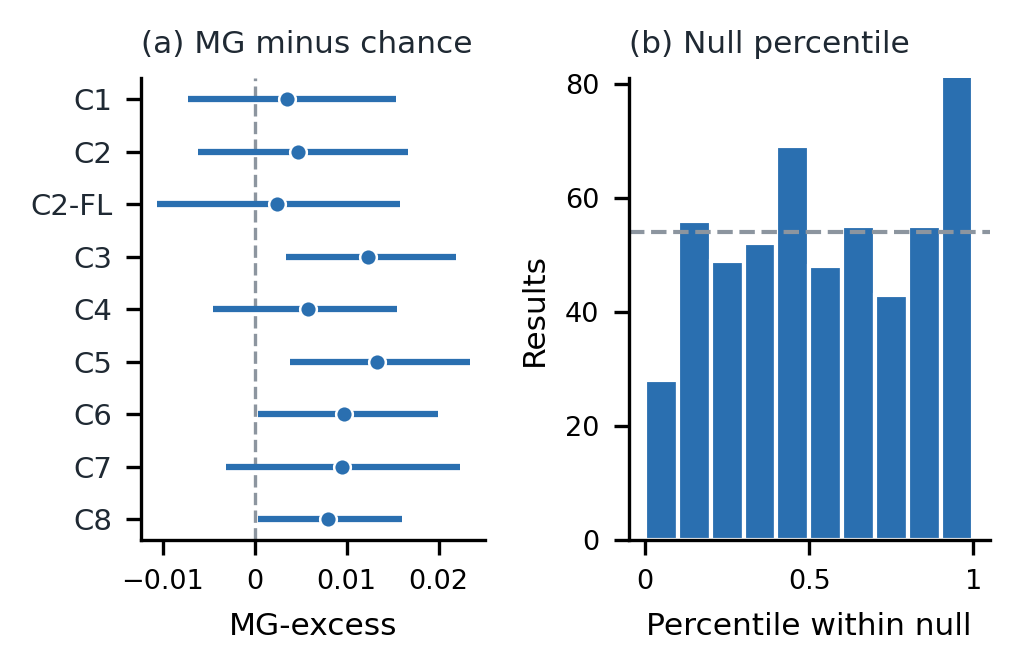
\includegraphics[width=\columnwidth]{fig11_null_calibration.png}
\caption{Null calibration of the baseline conditions (names in Table~\ref{tab:baseline}). (a) MG-excess with 95\% cluster-bootstrap CIs; dashed: chance (0). (b) Percentile of each per-client MG within its own null, for all 540 client--seed--condition results; dashed: the count expected by chance. Real masking would pile up near 1.}
\label{fig:null}
\end{figure}

\emph{Why the noise is so large.} The null 95th percentile of MG drops below 0.10 only at about 300 test records per client, and below 0.05 only above 1,000 (Fig.~\ref{fig:power}); our clients have 37--141. The minimum over seven AUCs picks whichever dimension happens to be estimated worst, which favors dimensions with few cases: 30--45\% of clients have too few Mental cases for any AUC. Which dimension is worst is only partly systematic: Sleep is the minimum in 22.0\% of results, against 16.0\% under the null. Eq.~(\ref{eq:closed}) gives 250 and 1,000 records for gaps of 0.10 and 0.05, within 12\% of the exact values (290 and 1,150).

\begin{figure}[t]
\centering
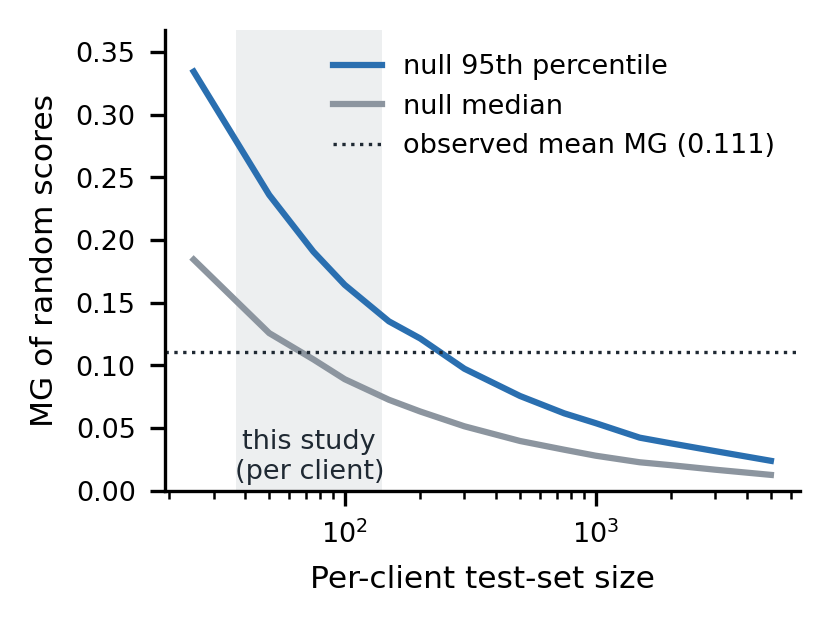
\includegraphics[width=0.82\columnwidth]{fig12_power_curve.png}
\caption{Median and 95th percentile of MG for random scores versus per-client test size, at this sample's prevalences. Shaded: the per-client test sizes in this study; dotted: mean observed MG over the baseline conditions.}
\label{fig:power}
\end{figure}

\emph{Comparing conditions.} With clients as units, no condition differs in MG from its reference: C2 versus C1, C3 versus C1, and C2-FL, C6, C7 and C8 versus C3 all have Holm $p = 1.00$ (e.g., C2-FL versus FedAvg, Hodges--Lehmann $-0.010$ [$-0.027$, $0.005$]), and the mixed model finds no condition different from FedAvg ($p \geq 0.23$). Read with fixed cut-points instead, the same numbers would label about half of all client results as masked under every method.

\subsection{Baseline population audit: federated outputs fall to chance}

Pooling clients removes most of the noise (null population MG: mean 0.027, 95th percentile 0.038). Table~\ref{tab:popauc} gives the client-averaged AUC per dimension. The centralized model is above chance on all seven dimensions (0.56--0.64). Under every federated condition, Sleep (0.49--0.52) and Mental (0.49--0.52) fall to chance, and FedAvg is above chance on only two of seven dimensions. This is a real failure of the baseline pipeline, and population MG misses it: no condition's population MG exceeds chance after Holm correction ($p \geq 0.16$; 0.033--0.043 for federated conditions), because MG measures the spread between dimensions, and when most dimensions sit near chance that spread is small. Only checking each dimension against chance finds the failure. Section~\ref{sec:full} traces it to unscaled inputs.

\begin{table}[t]
\caption{Client-averaged AUC per dimension, baseline conditions (3 seeds). $^{*}$: 95\% cluster-bootstrap CI above 0.5.}
\label{tab:popauc}
\centering\small
\setlength{\tabcolsep}{2.2pt}
\begin{tabular}{@{}lccccccc@{}}
\toprule
 & Sleep & Act. & Sed. & Ment. & Metab. & Wellb. & Diet \\
\midrule
C1    & .557$^{*}$ & .588$^{*}$ & .554$^{*}$ & .571$^{*}$ & .638$^{*}$ & .610$^{*}$ & .574$^{*}$ \\
C2    & .562$^{*}$ & .584$^{*}$ & .548$^{*}$ & .534 & .628$^{*}$ & .588$^{*}$ & .569$^{*}$ \\
C2-FL & .509 & .529$^{*}$ & .535$^{*}$ & .489 & .575$^{*}$ & .545$^{*}$ & .522$^{*}$ \\
C3    & .495 & .518 & .503 & .504 & .568$^{*}$ & .529$^{*}$ & .509 \\
C4    & .488 & .531$^{*}$ & .510 & .486 & .539$^{*}$ & .523 & .500 \\
C5    & .496 & .494 & .511 & .506 & .567$^{*}$ & .532$^{*}$ & .509 \\
C6    & .520 & .533$^{*}$ & .525 & .517 & .556$^{*}$ & .556$^{*}$ & .505 \\
C7    & .502 & .504 & .512 & .509 & .556$^{*}$ & .508 & .509 \\
C8    & .494 & .488 & .514 & .516 & .540$^{*}$ & .558$^{*}$ & .527$^{*}$ \\
\bottomrule
\end{tabular}
\end{table}

\subsection{Full protocol: the federated failure comes from unscaled inputs}\label{sec:full}

Fig.~\ref{fig:regimes} shows the per-dimension audit on the pooled test set for the baseline and the full protocol. The full protocol lifts FedAvg's macro-AUC from 0.518 to 0.643 and moves every dimension above chance (Sleep 0.497 $\rightarrow$ 0.613, Mental 0.505 $\rightarrow$ 0.643, Wellbeing 0.488 $\rightarrow$ 0.706). An ablation on seeds 42, 123 and 456 attributes the whole gain to preprocessing: standardized inputs with one-hot race/ethnicity reach 0.639 even with the baseline learning rate and the final round, whereas validation-based checkpoints and the tuned learning rate on raw inputs reach only 0.517. In the baseline, FedAvg trained on unscaled inputs (ages near 50, blood pressure near 120, category codes 1--7) whose distributions differ across clients; centralized training tolerated this and federated averaging did not. With standardized inputs, federation costs 0.008 macro-AUC (95\% CI [0.006, 0.010], lower on all 10 seeds, Holm $p<10^{-3}$; at most 0.013 on any dimension) and no dimension falls to chance. Richer features raise macro-AUC to 0.697 (C1) and 0.689 (C3), most for Mental, Metabolic and Wellbeing (+0.07 to +0.09).

The other aggregation schemes behave as follows (Table~\ref{tab:summary}). Standard SCAFFOLD closes the remaining gap (macro-AUC $+0.007$ over FedAvg with both feature sets, Holm $p<10^{-3}$, level with C1); Ditto's personalized models with the tuned $\lambda{=}1$ add 0.004 (Holm $p \leq 0.01$); and CS-Agg, q-FedAvg, FedProx and C8 stay within 0.003 of FedAvg. The per-dimension audit did its job: it exposed a preprocessing problem that neither the composite score nor per-client MG could reveal.

\begin{figure*}[t]
\centering
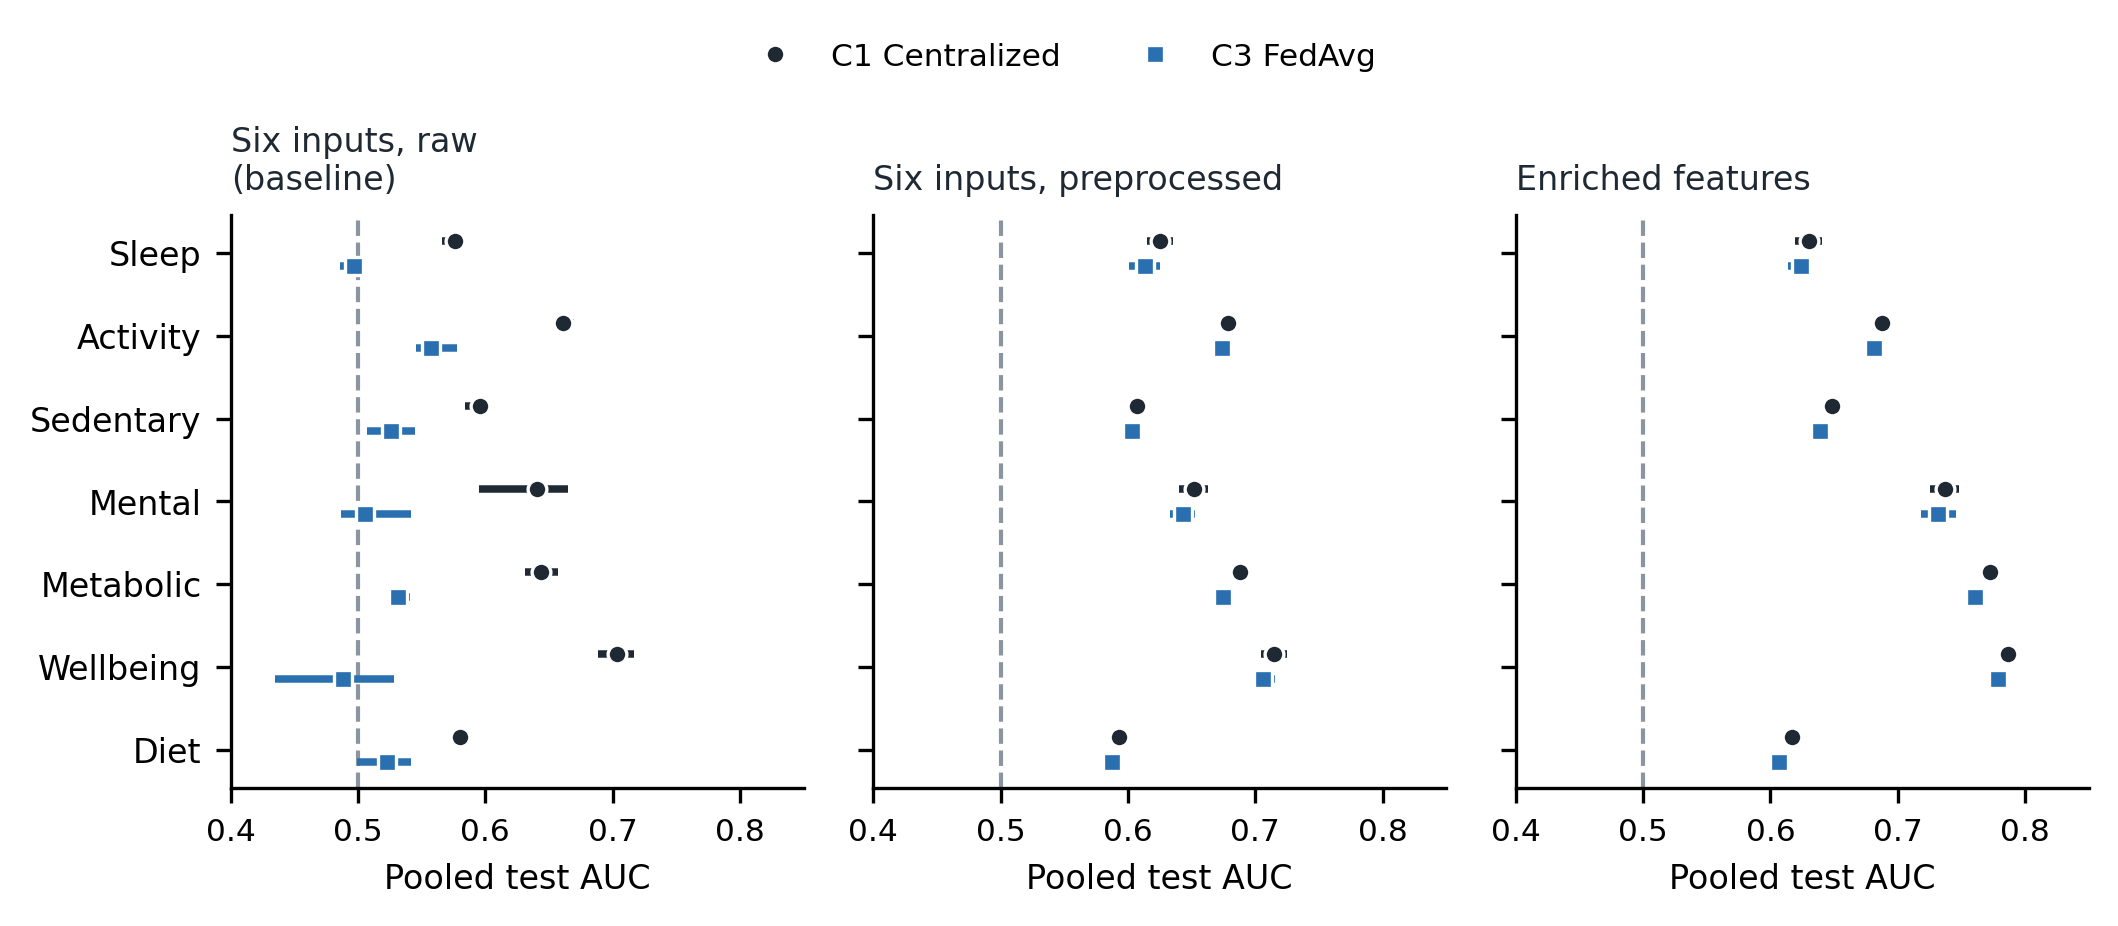
\includegraphics[width=0.86\textwidth]{fig13_dimension_auc_by_regime.png}
\caption{Pooled test AUC per dimension (mean and 95\% CI over seeds) for centralized (C1) and FedAvg (C3) training: the baseline with raw inputs (3 seeds), and the full protocol with the six base inputs preprocessed and with the enriched feature set (10 seeds each). Dashed: chance.}
\label{fig:regimes}
\end{figure*}

\begin{table}[t]
\caption{Summary of the baseline and full protocol (pooled test set, mean over seeds). Macro: AUC averaged over dimensions. Min: worst dimension's AUC. Pooled MG: its chance 95th percentile is about 0.04. MG-exc.: per-client MG minus its label-permutation null ($^{*}$ Holm $p<0.05$ across all 30 conditions analyzed, clients as units). $\bar\Delta$: blind spot averaged over dimensions. ECE: expected calibration error.}
\label{tab:summary}
\centering\small
\setlength{\tabcolsep}{2.6pt}
\begin{tabular}{@{}lcccccc@{}}
\toprule
Condition & Macro & Min & Pooled MG & MG-exc. & $\bar\Delta$ & ECE \\
\midrule
\multicolumn{7}{@{}l}{\emph{Baseline (six raw inputs, 3 seeds)}} \\
C1 & 0.629 & 0.574 & 0.055 & $+0.004$ & 0.063 & 0.032 \\
C3 FedAvg & 0.518 & 0.469 & 0.049 & $+0.013$ & 0.037 & 0.039 \\
\multicolumn{7}{@{}l}{\emph{Full protocol, six inputs preprocessed (10 seeds)}} \\
C1 & 0.651 & 0.592 & 0.059 & $+0.010$ & 0.070 & 0.020 \\
C2 & 0.650 & 0.591 & 0.059 & $+0.010$ & 0.069 & 0.021 \\
C3 FedAvg & 0.643 & 0.586 & 0.058 & $+0.011$ & 0.067 & 0.024 \\
C2-FL & 0.644 & 0.584 & 0.060 & $+0.012$ & 0.068 & 0.026 \\
C4 SCAFFOLD & 0.651 & 0.593 & 0.058 & $+0.007$ & 0.069 & 0.022 \\
C5 CS-Agg & 0.643 & 0.584 & 0.059 & $+0.009$ & 0.066 & 0.024 \\
C6 Ditto & 0.647 & 0.588 & 0.060 & $+0.009$ & 0.068 & 0.021 \\
C7 q-FedAvg & 0.642 & 0.585 & 0.057 & $+0.009$ & 0.065 & 0.024 \\
C8 & 0.643 & 0.586 & 0.057 & $+0.010$ & 0.068 & 0.023 \\
C9 FedProx & 0.644 & 0.585 & 0.059 & $+0.010$ & 0.067 & 0.028 \\
C3 + class wt. & 0.627 & 0.574 & 0.053 & $+0.008$ & 0.053 & 0.170 \\
C3 + focal & 0.641 & 0.582 & 0.059 & $+0.011^{*}$ & 0.064 & 0.108 \\
\multicolumn{7}{@{}l}{\emph{Full protocol, enriched features (10 seeds)}} \\
C1 & 0.697 & 0.615 & 0.083 & $+0.023^{*}$ & 0.078 & 0.027 \\
C2 & 0.695 & 0.612 & 0.083 & $+0.024^{*}$ & 0.076 & 0.030 \\
C3 FedAvg & 0.689 & 0.604 & 0.084 & $+0.024^{*}$ & 0.073 & 0.023 \\
C2-FL & 0.688 & 0.607 & 0.082 & $+0.023^{*}$ & 0.073 & 0.029 \\
C4 SCAFFOLD & 0.696 & 0.611 & 0.085 & $+0.022^{*}$ & 0.077 & 0.022 \\
C5 CS-Agg & 0.688 & 0.606 & 0.083 & $+0.023^{*}$ & 0.073 & 0.031 \\
C6 Ditto & 0.692 & 0.607 & 0.086 & $+0.023^{*}$ & 0.074 & 0.028 \\
C7 q-FedAvg & 0.688 & 0.605 & 0.083 & $+0.024^{*}$ & 0.073 & 0.030 \\
C8 & 0.686 & 0.603 & 0.083 & $+0.023^{*}$ & 0.073 & 0.030 \\
C9 FedProx & 0.687 & 0.604 & 0.083 & $+0.023^{*}$ & 0.073 & 0.030 \\
C3 + class wt. & 0.674 & 0.601 & 0.074 & $+0.024^{*}$ & 0.060 & 0.144 \\
C3 + focal & 0.686 & 0.601 & 0.084 & $+0.023^{*}$ & 0.070 & 0.111 \\
\bottomrule
\end{tabular}
\end{table}

\subsection{Per-client masking grows with signal but stays small}

Table~\ref{tab:summary} shows how per-client MG changes as the models improve. With the six preprocessed inputs, MG-excess is $+0.007$ to $+0.012$, and only C3 with focal loss differs from chance after Holm correction ($p=0.037$). With richer features, the dimensions separate more (pooled MG about 0.08, against a chance 95th percentile of about 0.04), and an excess of $+0.022$ to $+0.024$ appears in every condition (Holm $p \leq 0.001$; 9.0--13.5\% of client results above the null 95th percentile). Even so, this real excess is about a fifth of the raw per-client MG (0.12--0.13); the rest is noise. A calibrated statistic shows this dose--response; raw MG cannot, since it stays at 0.11--0.13 in every regime.

Population-level MG exceeds its chance 95th percentile in every full-protocol configuration on average over seeds (in 90--100\% of individual seeds), centralized training included. It reflects how unevenly learnable the seven dimensions are from these inputs, not something federated training causes. Whether the composite \emph{hides} that unevenness is a separate question, answered in Section~\ref{sec:blind}.

\emph{Other partitions.} The results do not depend on the income-by-age clients. With a random split into 20 equal clients (65--109 test records each), raw MG is 0.11--0.13 against a chance level of 0.100, and MG-excess is $+0.011$ (six inputs) and $+0.024$ to $+0.025$ (enriched). With 12 race/ethnicity $\times$ sex clients (24--332 records) the excess is largest, $+0.030$ to $+0.032$ and $+0.043$, and the same for centralized predictions grouped the same way, so it reflects differences between demographic groups in the data, not federation. Under all three partitions, FedAvg stays within 0.009 macro-AUC of centralized training and $\Delta_d$ stays between 0.02 and 0.15.

\subsection{The composite score hides every dimension's signal}\label{sec:blind}

In every full-protocol configuration and every dimension, the composite flags poor cases worse than the dimension's own output: $\Delta_d$ ranges from 0.015 to 0.157 AUC, and the 95\% CIs over seeds exclude zero in all 196 configuration--dimension pairs (Fig.~\ref{fig:blind}). The loss is largest for Sedentary (0.10--0.16) and Activity (0.05--0.10) and smallest for Metabolic (0.02--0.05), and it is similar for every aggregation scheme and loss (0.06--0.07 averaged over dimensions). In the baseline FedAvg runs, $\Delta_d$ was small for Sleep, Mental, Wellbeing and Diet ($-0.016$ to $+0.029$), but only because those outputs carried little signal to hide.

\begin{figure}[t]
\centering
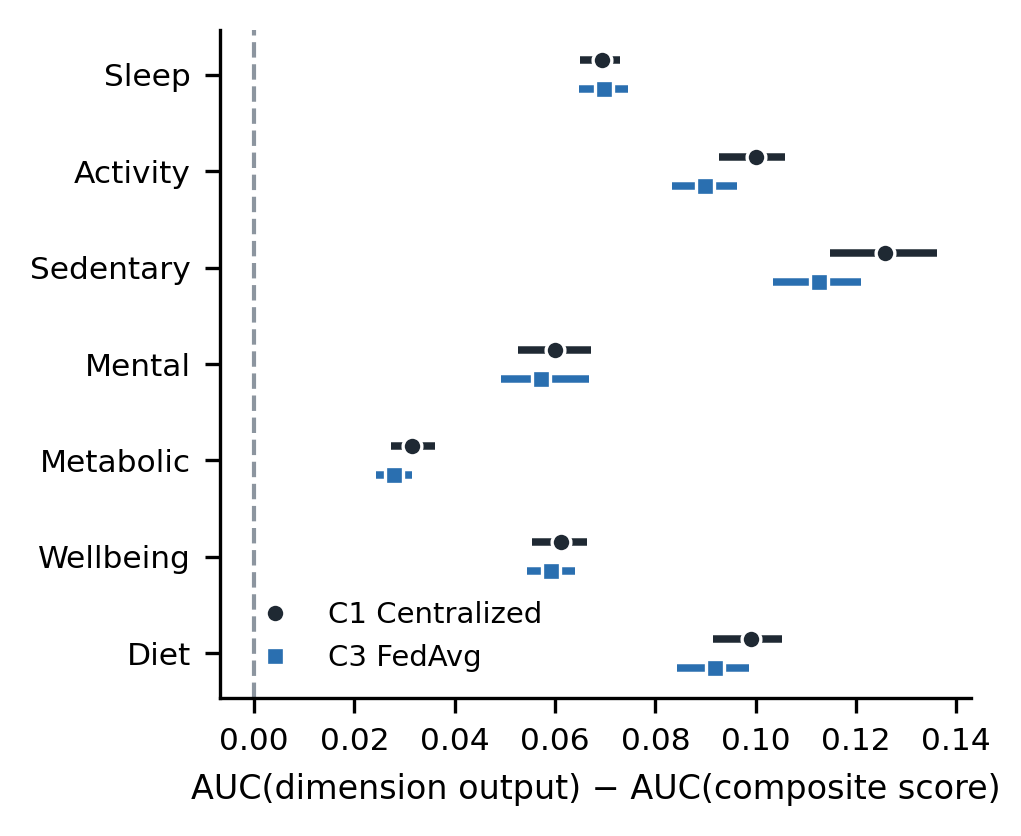
\includegraphics[width=0.92\columnwidth]{fig14_composite_blind_spot.png}
\caption{Composite blind spot $\Delta_d$ (enriched features, 10 seeds, 95\% CI): how much worse the composite score is than the dimension's own output at flagging that dimension's poor cases.}
\label{fig:blind}
\end{figure}

\subsection{Class imbalance, thresholds and decoupled training}

At the default 0.5 threshold, models trained with plain cross-entropy almost never flag Sleep (TPR 0.00--0.02) or Mental (0.00--0.03). With a threshold tuned on validation data, the same models reach TPR 0.51--0.62 for Sleep and 0.57--0.70 for Mental, and mean balanced accuracy rises from 0.55 to 0.60 (preprocessed inputs) and from 0.58 to 0.64 (enriched). Near-zero sensitivity at 0.5 is a threshold artifact, not a property of the training objective.

Class weighting moves the default operating point (Sleep TPR 0.54--0.61 at 0.5), but it lowers FedAvg macro-AUC by 0.014--0.017 (all 10 seeds) and raises ECE from about 0.02 to 0.14--0.17. Focal loss changes AUC by at most 0.004 and raises ECE to about 0.11. Training each dimension as a separate federation (C2-FL) costs seven times FedAvg's communication, yet it does not differ from FedAvg on macro-AUC, worst-dimension AUC or pooled MG in either feature set (all $|\text{difference}| \leq 0.003$, Holm $p \geq 0.81$). More broadly, no aggregation scheme or decoupled objective changes pooled MG relative to its reference; of 26 paired comparisons, only class weighting with enriched features lowers it ($-0.011$, Holm $p=0.002$), and it does so while lowering macro-AUC by 0.014 (all others $|\text{difference}| \leq 0.005$, Holm $p \geq 0.81$).

\subsection{Subgroup fairness and attribution stability}

Masking also occurs across demographic groups. Across the plain cross-entropy configurations with preprocessed inputs, the AUC gap between income groups is largest for Mental (0.15--0.20) and Wellbeing (0.10--0.12), and the worst income group's Mental AUC is at chance (0.46--0.49). Richer features narrow the Mental gap to 0.13--0.14 and raise the worst group to 0.63--0.67. One global threshold turns these gaps into large equal-opportunity violations: Mental sensitivity differs between income groups by 0.78--0.84 and Wellbeing by 0.82--0.86 (0.38--0.55 and 0.42--0.50 with richer features), because prevalence falls steeply with income. Federated and centralized training behave alike here.

\emph{Attribution stability.} We computed SHAP attributions~\cite{lundberg2017} (GradientExplainer, 100 background and 300 explained test records) for the centralized model of every seed. For multi-column feature groups such as race/ethnicity, we sum each person's signed contributions before averaging their magnitude. Group rankings agree closely across seeds (Kendall's $W$ = 0.90--0.99 with the six inputs, 0.78--0.95 with richer features), and each dimension's top group is the same in 50--100\% of seeds. Effect directions match established epidemiology in all ten seeds: a lower poverty-income ratio raises predicted risk of depression~\cite{lorant2003} and of fair/poor self-rated health~\cite{braveman2014}, older age raises risk of insufficient activity, and male sex raises risk of above-median sugar intake. With richer features, prescription count leads for Mental and cholesterol (total and HDL) for Metabolic in every seed, while education and prescription count split the lead for Wellbeing (5 vs.\ 5 of 10). A single seed can mislead: for Metabolic with the six inputs, systolic blood pressure and race/ethnicity swap the top rank across seeds (6 vs.\ 4 of 10).

\section{Discussion}

\emph{What the composite hides.} The composite can hide two different problems, and each needs its own audit. When a dimension carries signal, the composite detects it worse than the model's own output for that dimension (positive $\Delta_d$); showing the per-dimension outputs next to the composite removes this loss at no cost. When federated training fails to learn a dimension at all (Sleep and Mental in the baseline), $\Delta_d$ is small because there is little left to hide, and only a per-dimension AUC audit catches the failure. Comparing per-client MG with a fixed cut-point catches neither.

\emph{Clinical relevance.} All labels except Diet use published cut-points (Table~\ref{tab:dims}). An AUC of 0.5 means no discrimination, and under one commonly cited descriptive convention 0.7--0.8 is termed acceptable~\cite{mandrekar2010}; these bands are not clinical-utility thresholds. Validated screeners such as the PHQ-9 do far better~\cite{kroenke2001}. Most per-dimension AUCs here are below 0.7 and none exceeds 0.8 when averaged over seeds, so none of these models is fit for screening individuals, masked or not. We therefore present MG as an \emph{audit} statistic whose severity is judged against sampling noise, not as a clinical-utility threshold; no guideline defines one for composite health scores.

\emph{Recommendations for auditing composite health models under FL.}
(i) Report MG with its chance level (MG-excess and null percentile), never raw. (ii) Plan per-client test sets with Eq.~(\ref{eq:closed}) (here about 300 records to resolve a gap of 0.10); audit smaller clients pooled or grouped. (iii) Treat AUCs with fewer than 5 cases of either class as missing, not as 0.5. (iv) Check each dimension's population AUC against chance and against a centralized model; an output at chance is a failure whatever the MG. (v) Report sensitivity at a validation-tuned threshold; at 0.5 it mostly reflects prevalence. (vi) Report $\Delta_d$ to show how much the composite hides.

\emph{Limitations.} NHANES is cross-sectional survey and exam data, not continuous wearable streams, so AUCs are modest and the results describe a setting with little information per person. The federations are simulated (three partitions of one survey, synchronous rounds), and survey weights are not applied. The random-score null treats dimensions as independent; the label-permutation null, used for the full protocol, keeps their dependence. Ditto's selected $\lambda$ was the largest value tried (1). Diet uses a sample-median split.

\section{Conclusion}

On per-client test sets this small, a raw Masking Gap cannot tell masking from noise: here it was 0.11--0.13 whether or not real differences between dimensions existed. Three tools separate what the raw statistic mixes together. Calibrating MG against chance removes estimation noise, a per-dimension population audit finds dimensions a model fails to learn, and the composite blind spot measures signal the composite hides. In our data, noise dominated per-client MG in the baseline; the failed dimensions were real but caused by unscaled inputs; and the hidden signal held across centralized training, seven federated schemes, loss functions, feature sets and client partitions. Composite wellness scores should be released with their per-dimension outputs and audited with calibrated statistics.

\section*{Data and Code Availability}
NHANES 2015--2018 is public~\cite{nhanes2015}. Code to rebuild the splits, features, experiments, null distributions, tables and figures will be released upon acceptance (anonymized for review).



\begin{thebibliography}{99}
\bibitem{doherty2025} C.~Doherty et al., ``Readiness, recovery, and strain: an evaluation of composite health scores in consumer wearables,'' \emph{Transl.\ Exerc.\ Biomed.}, vol.~2, no.~2, pp.~128--144, 2025.
\bibitem{whoop2024} Whoop, ``Whoop 101: Recovery,'' 2024. [Online]. Available: \url{https://developer.whoop.com/docs/whoop-101/}. Accessed: Sep.~26, 2026.
\bibitem{garmin2024} Garmin, ``Body Battery energy monitor,'' 2024. [Online]. Available: \url{https://www.garmin.com/en-US/garmin-technology/health-science/body-battery/}. Accessed: Sep.~26, 2026.
\bibitem{oura2024} Oura, ``Readiness contributors,'' Oura Member Care, 2024. [Online]. Available: \url{https://support.ouraring.com/hc/en-us/articles/360057791533-Readiness-Contributors}. Accessed: Sep.~26, 2026.
\bibitem{nhanes2015} Centers for Disease Control and Prevention, ``National Health and Nutrition Examination Survey data, 2015--2018,'' U.S.\ Dept.\ of Health and Human Services. [Online]. Available: \url{https://www.cdc.gov/nchs/nhanes}. Accessed: Sep.~26, 2026.
\bibitem{rieke2020} N.~Rieke et al., ``The future of digital health with federated learning,'' \emph{npj Digit.\ Med.}, vol.~3, p.~119, 2020.
\bibitem{mcmahan2017} B.~McMahan, E.~Moore, D.~Ramage, S.~Hampson, and B.~A.~y~Arcas, ``Communication-efficient learning of deep networks from decentralized data,'' in \emph{Proc.\ AISTATS}, 2017, pp.~1273--1282.
\bibitem{grataloup2024} A.~Grataloup and M.~Kurpicz-Briki, ``A systematic survey on the application of federated learning in mental state detection and human activity recognition,'' \emph{Front.\ Digit.\ Health}, vol.~6, p.~1495999, 2024.
\bibitem{li2020fedprox} T.~Li et al., ``Federated optimization in heterogeneous networks,'' in \emph{Proc.\ MLSys}, 2020, pp.~429--450.
\bibitem{karimireddy2020} S.~P.~Karimireddy et al., ``SCAFFOLD: Stochastic controlled averaging for federated learning,'' in \emph{Proc.\ ICML}, 2020, pp.~5132--5143.
\bibitem{li2021ditto} T.~Li, S.~Hu, A.~Beirami, and V.~Smith, ``Ditto: Fair and robust federated learning through personalization,'' in \emph{Proc.\ ICML}, 2021, pp.~6357--6368.
\bibitem{fallah2020} A.~Fallah, A.~Mokhtari, and A.~Ozdaglar, ``Personalized federated learning with theoretical guarantees: A model-agnostic meta-learning approach,'' in \emph{Proc.\ NeurIPS}, 2020, pp.~3557--3568.
\bibitem{li2020qfedavg} T.~Li, M.~Sanjabi, A.~Beirami, and V.~Smith, ``Fair resource allocation in federated learning,'' in \emph{Proc.\ ICLR}, 2020.
\bibitem{cao2021fltrust} X.~Cao, M.~Fang, J.~Liu, and N.~Z.~Gong, ``FLTrust: Byzantine-robust federated learning via trust bootstrapping,'' in \emph{Proc.\ NDSS}, 2021.
\bibitem{oakdenrayner2020} L.~Oakden-Rayner, J.~Dunnmon, G.~Carneiro, and C.~R\'e, ``Hidden stratification causes clinically meaningful failures in machine learning for medical imaging,'' in \emph{Proc.\ ACM CHIL}, 2020, pp.~151--159.
\bibitem{obermeyer2019} Z.~Obermeyer, B.~Powers, C.~Vogeli, and S.~Mullainathan, ``Dissecting racial bias in an algorithm used to manage the health of populations,'' \emph{Science}, vol.~366, no.~6464, pp.~447--453, 2019.
\bibitem{burnell2023} R.~Burnell et al., ``Rethink reporting of evaluation results in AI,'' \emph{Science}, vol.~380, no.~6641, pp.~136--138, 2023.
\bibitem{collins2024} G.~S.~Collins et al., ``TRIPOD+AI statement: updated guidance for reporting clinical prediction models that use regression or machine learning methods,'' \emph{BMJ}, vol.~385, e078378, 2024.
\bibitem{sener2018} O.~Sener and V.~Koltun, ``Multi-task learning as multi-objective optimization,'' in \emph{Proc.\ NeurIPS}, vol.~31, 2018.
\bibitem{chen2018gradnorm} Z.~Chen, V.~Badrinarayanan, C.-Y.~Lee, and A.~Rabinovich, ``GradNorm: Gradient normalization for adaptive loss balancing in deep multitask networks,'' in \emph{Proc.\ ICML}, 2018, pp.~794--803.
\bibitem{kendall2018} A.~Kendall, Y.~Gal, and R.~Cipolla, ``Multi-task learning using uncertainty to weigh losses for scene geometry and semantics,'' in \emph{Proc.\ CVPR}, 2018, pp.~7482--7491.
\bibitem{yu2020pcgrad} T.~Yu, S.~Kumar, A.~Gupta, S.~Levine, K.~Hausman, and C.~Finn, ``Gradient surgery for multi-task learning,'' in \emph{Proc.\ NeurIPS}, 2020, pp.~5824--5836.
\bibitem{lin2017focal} T.-Y.~Lin, P.~Goyal, R.~Girshick, K.~He, and P.~Doll\'ar, ``Focal loss for dense object detection,'' in \emph{Proc.\ ICCV}, 2017, pp.~2999--3007.
\bibitem{hanley1982} J.~A.~Hanley and B.~J.~McNeil, ``The meaning and use of the area under a receiver operating characteristic (ROC) curve,'' \emph{Radiology}, vol.~143, no.~1, pp.~29--36, 1982.
\bibitem{ojala2010} M.~Ojala and G.~C.~Garriga, ``Permutation tests for studying classifier performance,'' \emph{J.\ Mach.\ Learn.\ Res.}, vol.~11, pp.~1833--1863, 2010.
\bibitem{gpaq} World Health Organization, ``Global Physical Activity Questionnaire (GPAQ) analysis guide,'' Geneva: WHO. [Online]. Available: \url{https://cdn.who.int/media/docs/default-source/ncds/ncd-surveillance/gpaq-analysis-guide.pdf}. Accessed: Sep.~26, 2026.
\bibitem{who2020} World Health Organization, \emph{WHO Guidelines on Physical Activity and Sedentary Behaviour}. Geneva: WHO, 2020.
\bibitem{patel2010} A.~V.~Patel et al., ``Leisure time spent sitting in relation to total mortality in a prospective cohort of US adults,'' \emph{Am.\ J.\ Epidemiol.}, vol.~172, no.~4, pp.~419--429, 2010.
\bibitem{watson2015} N.~F.~Watson et al., ``Recommended amount of sleep for a healthy adult,'' \emph{Sleep}, vol.~38, no.~6, pp.~843--844, 2015.
\bibitem{kroenke2001} K.~Kroenke, R.~L.~Spitzer, and J.~B.~W.~Williams, ``The PHQ-9: Validity of a brief depression severity measure,'' \emph{J.\ Gen.\ Intern.\ Med.}, vol.~16, no.~9, pp.~606--613, 2001.
\bibitem{who2000} World Health Organization, ``Obesity: preventing and managing the global epidemic,'' WHO Tech.\ Rep.\ Ser.\ 894, Geneva, 2000.
\bibitem{idler1997} E.~L.~Idler and Y.~Benyamini, ``Self-rated health and mortality: a review of twenty-seven community studies,'' \emph{J.\ Health Soc.\ Behav.}, vol.~38, no.~1, pp.~21--37, 1997.
\bibitem{kingma2015} D.~P.~Kingma and J.~Ba, ``Adam: A method for stochastic optimization,'' in \emph{Proc.\ ICLR}, 2015.
\bibitem{mann1947} H.~B.~Mann and D.~R.~Whitney, ``On a test of whether one of two random variables is stochastically larger than the other,'' \emph{Ann.\ Math.\ Statist.}, vol.~18, no.~1, pp.~50--60, 1947.
\bibitem{youden1950} W.~J.~Youden, ``Index for rating diagnostic tests,'' \emph{Cancer}, vol.~3, no.~1, pp.~32--35, 1950.
\bibitem{hardt2016} M.~Hardt, E.~Price, and N.~Srebro, ``Equality of opportunity in supervised learning,'' in \emph{Proc.\ NIPS}, 2016, pp.~3315--3323.
\bibitem{wilcoxon1945} F.~Wilcoxon, ``Individual comparisons by ranking methods,'' \emph{Biometrics Bull.}, vol.~1, no.~6, pp.~80--83, 1945.
\bibitem{holm1979} S.~Holm, ``A simple sequentially rejective multiple test procedure,'' \emph{Scand.\ J.\ Statist.}, vol.~6, no.~2, pp.~65--70, 1979.
\bibitem{lundberg2017} S.~M.~Lundberg and S.-I.~Lee, ``A unified approach to interpreting model predictions,'' in \emph{Proc.\ NeurIPS}, 2017, pp.~4765--4774.
\bibitem{lorant2003} V.~Lorant, D.~Deli\`ege, W.~Eaton, A.~Robert, P.~Philippot, and M.~Ansseau, ``Socioeconomic inequalities in depression: a meta-analysis,'' \emph{Am.\ J.\ Epidemiol.}, vol.~157, no.~2, pp.~98--112, 2003.
\bibitem{braveman2014} P.~Braveman and L.~Gottlieb, ``The social determinants of health: it's time to consider the causes of the causes,'' \emph{Public Health Rep.}, vol.~129, suppl.~2, pp.~19--31, 2014.
\bibitem{mandrekar2010} J.~N.~Mandrekar, ``Receiver operating characteristic curve in diagnostic test assessment,'' \emph{J.\ Thorac.\ Oncol.}, vol.~5, no.~9, pp.~1315--1316, 2010.
\end{thebibliography}

\end{document}
